\chapter{Analysing Classes}
Python has two different kinds of classes, namely new and old style (or classic) classes that both support multiple inheritance. A new style class is one that contrary to an old style class is a subclass of \inlinecode{object}. The two different kinds of classes vary among others in their method resolution order (MRO) \cite{pyref.typehierarchy}: old style classes resolves variables and attributes by a depth-first, left-to-right strategy, whereas new style classes use the more complex strategy C3 \cite{pyref.c3mro}, which is also known as the call-next-method from other multiple inheritance languages. Since our motivation for supporting classes is to be able to analyse programs that use the magic method \inlinecode{\_\_getattr\_\_} we have only been working with classes that does not use inheritance. In this chapter we present our work towards handling class declarations, object creations, method invocations and attribute lookup on class instances for such classes.

%To start with consider the below example that illustrates the difference in MRO between new and old style classes.

%\begin{listing}[H]
%	\begin{minted}[linenos]{python}
%class A():
%	x = 'A'
%class B(A): pass
%class C(A):
%	x = 'C'
%class D(B, C): pass
%D().x # 'A'
%	\end{minted}
%	\caption{Multiple inheritance}\label{code:OldStyleMROExample}
%\end{listing}

%Since \inlinecode{D} extends \inlinecode{B} and \inlinecode{C}, which in turn extends the old style class \inlinecode{A}, \inlinecode{D} is itself an old style class. Therefore, evaluating \inlinecode{D().x} will result in \inlinecode{'A'}. If we instead had declared \inlinecode{A} as a new style class \inlinecode{class A(object): ...}, evaluating \inlinecode{D().x} would result in \inlinecode{'C'}.


\section{Class declarations}
In the CFG we have the following nodes related to class declarations: \textit{ClassDeclNode}, \textit{ClassEntryNode}, and \textit{ClassExitNode}. For \inlinecode{class C: <body>} we create a class declaration node in our CFG. Next, we create a class entry node which will become the successor of the class declaration node. Then, the inductively created CFG for \inlinecode{<body>} will be inserted after the class entry node, and finally, we create a class exit node and make it the successor of the exit node of the inductively created \inlinecode{<body>} CFG.

\begin{listing}[H]
	\begin{center}
		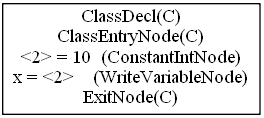
\includegraphics[width=0.5\textwidth]{images/class-decl-cfg.png}
	\end{center}
	\vspace{-10pt}
	\caption{The CFG generated by \inlinecode{class C: x = 10}.}
\end{listing}

The semantics of the three CFG nodes is the following:

\begin{itemize}
	\item The class declaration node, \textit{ClassDeclNode}, creates an empty class object on the abstract heap and writes the variable \inlinecode{C} as an attribute on the top object of the scope chain\footnote{Recall from \autoref{The Stack} that there may be more than one dynamic scope chain. In this case we write \inlinecode{C} to the top object of each scope chain.}.
	\item The class entry node, \textit{ClassEntryNode}, pushes the newly created class object onto the scope chain.
	\item The class exit node, \textit{ClassExitNode}, reverts the scope chain to what it looked like before visiting the class entry node by popping the newly created class object from the scope chain.
\end{itemize}

The class declaration node and the class entry node could in principle be turned into a single node. We chose to have the two nodes in order to have a clear distinction between when the class object is created and when it is populated.


\subsection{Populating the class objects with fields and methods}
When an empty class object has been created on the abstract heap due to a class declaration node, we add fields and methods to it inbetween the class entry node and the class exit node. Before we turn to how we do this, let us first investigate how fields and methods are created for classes in Python.

\begin{listing}[H]
	\begin{minted}[linenos]{python}
class C:
  x = 10
  def getX(self):
    return self.x
def setX(self, x):
  self.x = x
C.setX = setX
	\end{minted}
	\caption{Adding a field \inlinecode{x} and methods \inlinecode{getX} and \inlinecode{setX} on a class.}
	\label{code:FieldAndMethodOnClass}
\end{listing}

As \autoref{code:FieldAndMethodOnClass} illustrates, fields and methods can be created both at class declaration and later. Those being added at class declaration can be handled in the analysis by pushing the class object onto the scope chain at the class entry node: for \inlinecode{x=exp}, \inlinecode{x} is set to \inlinecode{exp} on the object on top of the scope chain (which will be the class object).

This is however not enough in order to support methods since our CFG cannot distinguish between function and method declarations. Thus \inlinecode{getX} will appear as a function declaration in our CFG, even though it is a method. We handle this at function declaration time in our analysis by checking whether the top of the scope chain is a class object. In that case we wrap the function in an unbound method object, which is merely just a pointer to the function object. Otherwise we proceed as we would otherwise have handled a function declaration as explained in \autoref{Functions} about functions.

We wrap the function in an unbound method object for at least two reasons:

\begin{enumerate}
	\item It is not possible to write attributes on methods, but attributes on methods can be read in case the underlying function has the attribute.
\end{enumerate}

This is illustrated by the following example:

\begin{listing}[H]
	\begin{minted}[linenos]{python}
class C: pass

def foo(self): pass
foo.attr = 42

C.foo = foo
C.foo.attr # 42
C.foo.attr = 0 # AttributeError
	\end{minted}
	\caption{It is not possible to set attributes on methods.}\label{code:FieldAndMethodOnClass}
\end{listing}

\begin{enumerate}
\setcounter{enumi}{1}
	\item When creating a class instance the unbound methods of the class are turned into bound methods on the instance object (we elaborate on this in \autoref{section: Handling object creations}, Handling object creations).
\end{enumerate}

Fields and methods can also be added to a class after declaration time as was illustrated in example \ref{code:FieldAndMethodOnClass}. In our CFG this is represented by a \textit{WriteVariableNode}. We handle this similar to what we do at class declaration: if the object being written to is a class object, and the value being written is a function, then we wrap it in an unbound method object. Otherwise we just write the value to the attribute of the object as we would otherwise have done.


\subsection{Handling object creations}
\label{section: Handling object creations}
In Python when a class instance is created each unbound method of the class is turned into a bound method on the object\todo{FORKERT}. The purpose of the bound method is to pass the instance reference as the first argument to the underlying function (the \inlinecode{self} argument):

\begin{listing}[H]
	\begin{minted}[linenos]{python}
class C(object):
  def foo(self):
    pass

C.foo # <unbound method C.foo>

x = C()
x.foo # <bound method C.foo of <C object at ...>>

x.foo() # self implicitly passed as self
C.foo(x) # using the unbound method by explicitly passing an instance

# TypeError: unbound method foo() must be called with C instance as 
# first argument (got nothing instead)
C.foo()
	\end{minted}
	\caption{Bound and unbound methods.}
	\label{code:BoundAndUnboundMethodsOnClass}
\end{listing}

As a consequence our lattice doesn't contain an explicit representation of the \inlinecode{this} object (unlike the lattice used by TAJS \cite{tajs}): we can simply treat \inlinecode{self} as a normal parameter to the function.

As can also be seen from \autoref{code:BoundAndUnboundMethodsOnClass}, class instances are not created using the \inlinecode{new} keyword. This means that we cannot necessarily distinguish a function call from an object creation. At each \textit{CallNode} in our CFG we therefore investigate which kind of object on the abstract heap is being called. If it is a class object that is being called, we create an instance object on the heap, representing the newly created instance. In particular, we do not modify the call graph as we do for function calls unless the magic method \inlinecode{\_\_init\_\_} has been implemented (see \autoref{section:Supporting constructor calls}, Supporting constructor calls, on how we handle this).

Consider the following code:

\begin{listing}[H]
	\begin{minted}[linenos]{python}
if (trickyComputation()):
	class C: pass
else:
	def C(): return 42
x = C()
	\end{minted}
	\caption{Difference between methods and functions on classes.}
	\label{code:BothNewOldClassAndFunction}
\end{listing}

For \autoref{code:BothNewOldClassAndFunction} it is not possible to tell whether \inlinecode{C} after the \inlinecode{if} statement is pointing to the class in line 2, or the function in line 4. Therefore, our analysis will conclude that \inlinecode{x} is either a pointer to a class instance, or the integer 42. This is seen in the figure below generated by our type analysis, which is the output of the heap at the exit node of the CFG of the code in example \ref{code:BothNewOldClassAndFunction}.

\begin{listing}[H]
	\begin{center}
		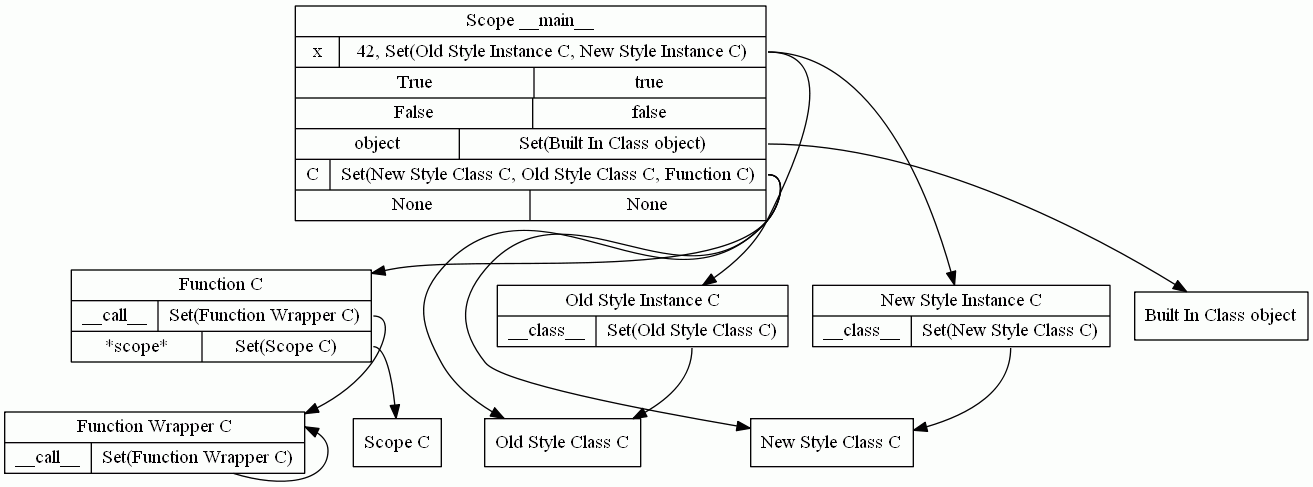
\includegraphics[width=1\textwidth]{images/BothNewOldClassAndFunction.png}
	\end{center}
	\vspace{-10pt}
	\caption{The heap generated by our analysis tool.}
	\label{fig:BothNewOldClassAndFunction}
\end{listing}


\section{Supporting constructor calls}
\label{section:Supporting constructor calls}
The magic method \inlinecode{\_\_init\_\_} can be set on a class in order to supply a constructor as the following illustrates:

\begin{listing}[H]
	\begin{minted}[linenos]{python}
class C(object):
	def __init__(self, x):
		self.x = x

c = C(42)
c.x # 42
	\end{minted}
	\caption{The \inlinecode{\_\_init\_\_} magic method.}\label{code:InitConstructorClass}
\end{listing}

This introduces a minor issue that arises from the fact that we cannot at first sight distinguish object creations from function invocations. What happens at line 5 in example \ref{code:InitConstructorClass} above is the following:

\begin{enumerate}
	\item A new style instance object is created on the heap because of the call to a new style class object.
	\item A value pointing to this newly created instance object is stored in the special return register on the stack.
	\item The call graph is updated with call edges from the call node to the entry node of \inlinecode{\_\_init\_\_}, and from the exit node of \inlinecode{\_\_init\_\_} to the after call node.
	\item As a result of (3), the return value of \inlinecode{\_\_init\_\_} is stored in the special return register. Note that the return value of \inlinecode{\_\_init\_\_} must be the built in constant \inlinecode{None}; otherwise a type error results (for this example our CFG will insert an implicit return \inlinecode{None} node).
	\item The after call node will now read the value from the special return register on the stack and store it; in this case as the attribute \inlinecode{x} of \inlinecode{c}.
\end{enumerate}

For this approach the best we can do is to take the least upper bound when we write to the special return register. As a consequence the variable \inlinecode{c} from the example will after the object creation be set to the value corresponding to either being \inlinecode{None} or a new style instance object (meaning that we should report a type error in line 6, because an attribute is possibly being dereferenced on a non-object!).

We solve this issue by introducing a new special constructor return register, where we store newly created class instances in, together with a new kind of call edge in the call graph; constructor call edges.

The idea is the following: Instead of updating the call graph with call edges in (3), we update it with constructor call edges. This means that we can recognize returns from \inlinecode{\_\_init\_\_} functions, check that they are indeed \inlinecode{\_\_None\_\_} (otherwise raise a type error) and then ignore it.

Specifically, our implementation has a special join operation for after call nodes (for all other nodes the join operation just takes the least upper bound of the solutions of its predecessors). This join operation for after call nodes is the usual join operation, except that solutions coming from constructor call edges have their special return register (containing \inlinecode{\_\_None\_\_} emptied). As a consequence, our analysis can just take the least upper bound of the values in the special return and the special constructor return register, respectively, and store it in e.g. the attribute \inlinecode{x} of \inlinecode{c}.


\section{Builtin classes}
To support some of the built-in function and classes Python contains, a specific \inlinecode{\_\_builtin\_\_.py} file is created and imported every time an analysis is made. This \inlinecode{\_\_builtin\_\_.py} file contains abstract implementations of the built-in function and classes written in Python. The idea of using the target language to implement some of the built-in functions is common in static analysis and can be seen in both the TAJS\cite{tajs} and the Lambda-py\cite{lambdapy} project, even though the projects have different approaches on how they do the static analysis.


\subsection{A note on handling both new and old style classes}
As mentioned we only handle classes that does not use inheritance in our analysis. If we were to handle both kinds of classes it would not be enough to only create one class object on the abstract heap for each class declaration.

\begin{itemize}
	\item If \inlinecode{C} is definitely a new style class a new style class object is created on the heap, likewise for old style classes.
	\item Otherwise, both a new style class object and an old style class object is created on the heap.
\end{itemize}

For the example in listing \ref{code:OldStyleMROExample} our analysis will only create an old style class object on the heap, however for the below example we generate two objects.

\begin{listing}[H]
	\begin{minted}[linenos]{python}
if (...):
	class B(): pass
else:
	class B(object): pass
class C(B): pass
	\end{minted}
	\caption{An example where we can't conclude that \inlinecode{C} is definitely a new style class or definitely an old style class.}\label{code:NotDefinatelyNewOldStyleClass}
\end{listing}

We conclude that a class is definitely a new style class if the following holds:

\begin{enumerate}
	\item The built in class \inlinecode{object} has not been overwritten.
\end{enumerate}

Of course it would still be possible to conclude that \inlinecode{class C(O): ...} is a new style class if the variable \inlinecode{O} has been set to \inlinecode{object} before overwriting \inlinecode{object} like in the below example.

\begin{listing}[H]
	\begin{minted}[linenos]{python}
O = object
object = 42
class C(O): pass
	\end{minted}
	\caption{The class \inlinecode{C} here is easily seen to be a new style class.}\label{code:ClassOverwrittenObject}
\end{listing}

However, our implementation does not at the moment check this because of the limited time of our project, and the fact that programmers should really not overwrite the built in \inlinecode{object}. Note that our implementation does conclude that \inlinecode{class C(O): ...} is a new style class if line 2 in the example had been skipped.

If \inlinecode{object} has not been overwritten, we check that:

\begin{enumerate}
\setcounter{enumi}{1}
	\item All the base classes \inlinecode{B1}, ..., \inlinecode{Bn} are either the built in object or definitely a new style class.
\end{enumerate}

Recall that the base classes \inlinecode{B1}, ..., \inlinecode{Bn} are just variable names. If \inlinecode{Bi} is the variable \inlinecode{object}, we can conclude that it is the built in object since we from (1) have that the built in \inlinecode{object} has not been overwritten. If \inlinecode{Bi} is not \inlinecode{object} we look up the variable on the scope chain, and make sure its value is only a pointer to a new style class object on the heap, or the built in class \inlinecode{object}. If it is for instance a pointer to either a new style class object or an old style class object (see for instance listing \ref{code:NotDefinatelyNewOldStyleClass}), we conclude that the class \inlinecode{C} it is not definitely a new style class object.

In the same way we conclude that a class is definitely an old style class.

\section{Further class work}
Not implemented yet: Resolution of methods and fields in super classes (specifically implementing the C3 MRO)\todo{Fixme}.

\section{Analyzing a concrete example}
Give a concrete example together with the output of our analysis tool on that particular example\todo{Fixme}.
